\section{Additional empirical results}\label{app:empirical}
\begin{table}[htbp]\centering\small
\caption{Leaving out one model family at a time}\label{tab:family}
\begin{tabular}{lrrr}
\toprule
Excluded family & $N$ & $\widehat\beta_2$ & s.e. \\
\midrule
Anthropic & 15,355 & -0.112 & 0.058 \\
DeepSeek & 23,385 & -0.044 & 0.060 \\
Google & 19,331 & -0.131 & 0.063 \\
OpenAI & 16,337 & -0.338 & 0.099 \\
Qwen & 21,166 & -0.102 & 0.065 \\
grok & 26,932 & -0.120 & 0.060 \\
kimi & 26,613 & -0.099 & 0.058 \\
llama & 23,015 & -0.028 & 0.068 \\
mistral & 23,681 & -0.053 & 0.062 \\
\bottomrule
\end{tabular}

\begin{minipage}{\textwidth}\footnotesize\vspace{0.5em}
Notes: Principal ECI matching rules, decisive first-round comparisons, with both sides in retained families. The coefficient multiplies the difference in squared centered ECI. Standard errors cluster by unordered model pair. Family exclusions change capability support and composition.
\end{minipage}
\end{table}

The ties robustness assigns half outcomes to ties and drops both-bad responses. It fits a fractional-outcome logit as a descriptive comparison rather than interpreting both-bad responses as indifference between acceptable models. The all-rounds specification admits repeated votes and receives less evidential weight. The GPQA exercise matches explicit benchmark model versions where available; its ECI counterpart uses identical comparisons. ECI and GPQA need not share evaluation budgets.

The crosswalk records unmatched and qualified entries rather than imputing their capability. Standard errors do not resolve mapping uncertainty. Nor does the analysis hold response style, speed, token use, or topic difficulty fixed. Identifying willingness to pay requires monetary choices or price variation with a demand model. Identifying developer profits further requires quantities, inference costs, research costs, financing, and complementary-product revenues.

\begin{table}[htbp]\centering\small
\caption{Dependence assumptions and descriptive uncertainty}\label{tab:inference}
\begin{tabular}{lrr}
\toprule
Coefficient & Pair-cluster s.e. & Dyadic s.e. \\
\midrule
Linear ECI & 0.05309 & 0.14454 \\
Quadratic ECI & 0.05706 & 0.15836 \\
\bottomrule
\end{tabular}

\end{table}
For the dyadic sensitivity, let $s_b$ be the individual logit score vector, $S_m$ its sum over comparisons incident to model $m$, and $S_{mn}$ its sum within unordered pair $\{m,n\}$. With inverse information matrix $A^{-1}$, the covariance is
\begin{equation}
 A^{-1}\left(\sum_m S_mS_m'-\sum_{m<n}S_{mn}S_{mn}'\right)A^{-1}.
\end{equation}
Each observation is included once per distinct endpoint model. Same-model comparisons have one endpoint and are not subtracted as a two-node overlap. No extra finite-model correction is applied. This permits dependence whenever comparisons share a model, while still excluding common shocks across unrelated models, uncertain capability scores, and selection into the matched sample. Finite dyadic estimates need not be positive semidefinite; the code reports eigenvalue diagnostics rather than silently treating this as definitive inference. With only 32 principal models, the normal intervals remain illustrative.

\begin{figure}[htbp]\centering
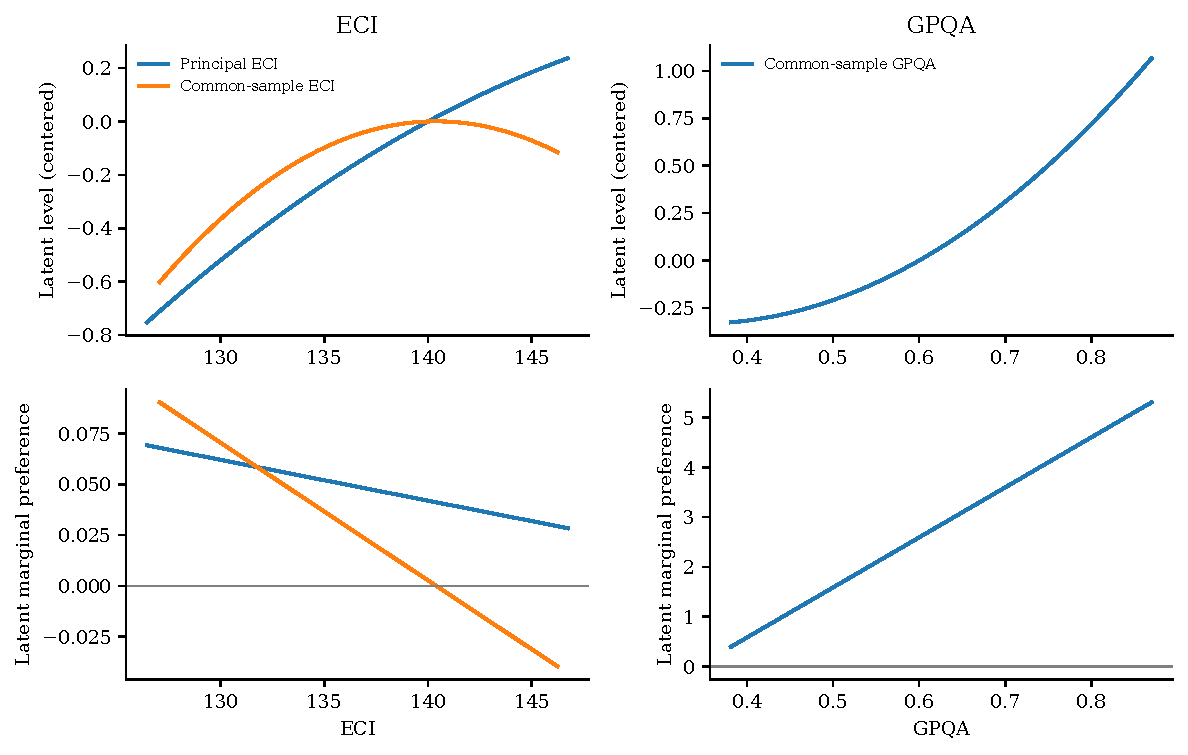
\includegraphics[width=.95\textwidth]{../output/figures/preference_support.pdf}
\caption{Fitted latent preference levels and slopes on observed support}\label{fig:support}
\begin{minipage}{\textwidth}\footnotesize
Notes: Levels omit the arbitrary utility constant and are centered using the regression's score normalization. Each curve is shown only on its own sample support. The ECI and GPQA common samples contain identical comparisons, but their capability measures can change model rankings, rather than merely transform a common ordering.
\end{minipage}
\end{figure}

In the common-sample ECI fit the marginal latent preference becomes negative above about 140.39, within support 127.07--146.24. It therefore does not represent positive but diminishing marginal value everywhere. The principal ECI fit's turning point lies above its own sample support. The contrast with GPQA can reflect both scale and changed model orderings; Lemma~\ref{lem:scale} applies only to a monotone relabeling of the entire same problem. The unconstrained quadratics are descriptive fits, not maintained utility functions for the theoretical game.

\clearpage
\section{Numerical assumptions and robustness}\label{app:parameters}
\begingroup\small\setstretch{1.0}
\begin{longtable}{p{0.23\textwidth}p{0.69\textwidth}}
\caption{Notation}\label{tab:notation}\\
\toprule Symbol & Meaning\\\midrule\endfirsthead
\toprule Symbol & Meaning\\\midrule\endhead
$i,j$ & Developer and jurisdiction indices.\\
$T,h$ & Total horizon and periods remaining.\\
$x,x',z$ & Current and updated controlled states; autonomous state.\\
$a_i,a$ & Developer and autonomous capability on a specified cardinal scale.\\
$K_i,F_i$ & Controlled research infrastructure and outside financing capacity.\\
$g_i,\mathcal G_i$ & Government policy and finite policy menu.\\
$b_i=(e_i,s_i,d_i)$ & Research, safety, and delegation action; $e_P$ is the fixed positive project input and $\kappa_s$ the safety infrastructure coefficient.\\
$R_\sigma,m,\sigma$ & Commercial benefits, their scale, and curvature.\\
$c_i,k_i,c_0,c_s,\gamma$ & Research and safety cost functions, normalized scales, cost exponent.\\
$S_i,\theta,v_i,\Gamma$ & Centered contest share, contest power, private and government positional scales.\\
$\ell_i,L,\chi$ & Private life flow, aggregate baseline human value, commercial surplus capture.\\
$q_i,q_{12},\omega_j$ & Individual and joint control-failure risks; selected-regime probabilities.\\
$P_0,P_j$ & Conditional no-failure controlled-state kernel and system-$j$ autonomous initial-state kernel.\\
$\beta,\beta_A$ & Human and autonomous discount factors.\\
$V_{i,h},Q_{i,h},W_{i,h}$ & Developer value, developer stage payoff, jurisdiction value.\\
$\pi,\pi^0$ & Development strategies and a restricted no-delegation equilibrium.\\
$G_s,G_d,Z_d,N,H$ & Supervised/delegated controlled continuation, failure continuation, net delegation gain, private failure loss.\\
$R_\infty,b,r,\xi,\lambda,K$ & Saturation level and gap, saturation exponent, recursive cost-decline exponent, proportional capability step, and its benefit coefficient in Proposition~\ref{prop:recursive}.\\
$\zeta,p_0$ & Research-input price exponent and scale in the recursive benchmark.\\
$\bar K,k,k_0,\underline H$ & Total resources, autonomous stock, initial stock, human subsistence stock.\\
$y,\kappa_y,a_S$ & Acquisition, its resource cost, and capability requirement.\\
$\rho,u_A,J_h$ & Containment probability, autonomous capability reward, autonomous value.\\
$g(k),\nu,L_h,N_h$ & Human production index, elasticity, post-loss human value, safe annuity.\\
$D_h,\tau,\mu^\pi_t$ & Autonomous extinction probability, first-loss date, first-loss state distribution.\\
$\tau_H,\tau_A$ & Human and autonomous terminal-value coefficients.\\
$\eta,\alpha,\phi,\psi,B_R,\mu_D$ & Research rate, input elasticity, assistance, difficulty, bottleneck, delegation multiplier.\\
$E,z_{mb},\delta,\beta_1,\beta_2$ & ECI, centered/scaled score, side effect, empirical preference coefficients.\\
\bottomrule
\end{longtable}
\endgroup
\begin{table}[H]\centering\small
\caption{Principal normalized reference assumptions}
\begin{tabular}{lrl}
\toprule
Replication parameter & Reference value & Status \\
\midrule
\texttt{beta} & 0.96 & Scenario assumption \\
\texttt{beta\_ai} & 0.98 & Scenario assumption \\
\texttt{sigma} & 1.3 & Scenario assumption \\
\texttt{commercial\_scale} & 1.0 & Scenario assumption \\
\texttt{prize} & 1.0 & Scenario assumption \\
\texttt{research\_cost} & 0.25 & Scenario assumption \\
\texttt{cost\_exponent} & 0.8 & Scenario assumption \\
\texttt{research\_eta} & 0.4 & Scenario assumption \\
\texttt{delegation\_multiplier} & 2.5 & Scenario assumption \\
\texttt{research\_feedback} & 0.9 & Scenario assumption \\
\texttt{research\_difficulty} & 0.5 & Scenario assumption \\
\texttt{q0} & 0.03 & Scenario assumption \\
\texttt{safety\_effect} & 2.0 & Scenario assumption \\
\texttt{containment} & 0.08 & Scenario assumption \\
\texttt{terminal\_years} & 5.0 & Scenario assumption \\
\bottomrule
\end{tabular}

\begin{minipage}{\textwidth}\footnotesize\vspace{0.5em}
Notes: All values in this table are scenario assumptions. Empirical bridges replace the cost exponent and research rate with \CostSlope\ and \BridgeEta, subject to the explicit mapping restrictions in Section~\ref{sec:evidence}. The complete parameter file specifies resources, budgets, meshes, and thresholds. Control-failure risk is not estimated.
\end{minipage}
\end{table}

\begin{table}[H]\centering\scriptsize
\caption{Sensitivity of the selected open-development equilibrium}\label{tab:sensitivity}
\resizebox{\textwidth}{!}{\begin{tabular}{lrrr}
\toprule
Specification & Loss of control (\%) & Extinction (\%) & Boundary (\%) \\
\midrule
5 years & 4.424 & 0.000 & 0.0000 \\
25 years & 4.576 & 4.358 & 0.0000 \\
25 years, no acquisition & 5.049 & 0.000 & 0.0000 \\
25 years, full common loss shock & 2.719 & 2.594 & 0.0000 \\
25 years, high-risk pure selection & 4.800 & 4.581 & 0.0000 \\
25 years, half capability mesh & 4.561 & 4.353 & 0.0000 \\
25 years, double capability ceiling & 4.576 & 4.358 & 0.0000 \\
25 years, zero terminal values & 4.243 & 4.025 & 0.0000 \\
25 years, long terminal values & 5.947 & 4.725 & 0.0000 \\
25 years, human terminal only zero & 4.243 & 4.026 & 0.0000 \\
25 years, AI terminal only zero & 4.576 & 4.358 & 0.0000 \\
25 years, post-containment recovery & 4.565 & 4.348 & 0.0000 \\
25 years, acquisition budget boundary & 4.574 & 4.357 & 0.0000 \\
25 years, no containment & 4.574 & 4.574 & 0.0000 \\
25 years, no positional prize & 3.211 & 3.001 & 0.0000 \\
25 years, low research feedback & 4.357 & 3.871 & 0.0000 \\
25 years, high research feedback & 3.786 & 3.692 & 0.0000 \\
bridge, half cost slope & 0.810 & 0.000 & 0.0000 \\
bridge, double finance & 0.000 & 0.000 & 0.0000 \\
bridge, ready to delegate & 0.810 & 0.000 & 0.0000 \\
bridge, higher market scale & 0.000 & 0.000 & 0.0000 \\
bridge, quarter-size projects & 1.816 & 0.000 & 0.0000 \\
bridge, quarter-size projects, 25 years & 1.816 & 1.816 & 0.0000 \\
cost bridge only & 0.812 & 0.000 & 0.0000 \\
progress bridge only & 0.810 & 0.000 & 0.0000 \\
\bottomrule
\end{tabular}
}
\begin{minipage}{\textwidth}\footnotesize\vspace{0.5em}
Notes: Long-horizon sensitivities use twenty-five years, bridge sensitivities ten years. Boundary is the probability of capability clipping at a computational ceiling. An all-path envelope fixes the domain before solving, covering deviations as well as selected paths. Zero within-horizon risk does not guarantee infinite-horizon safety. Selection sensitivities compare specified equilibria, not the complete correspondence.
\end{minipage}
\end{table}

The support solver verifies that supported actions are best responses and excluded actions do not improve payoffs. Linear feasibility programs accommodate unequal supports and degenerate games. Probability recursions are undiscounted; payoff recursions are discounted. Keeping them separate prevents interpreting discounted hazards as extinction probabilities.

The numerical certificate separately solves the restricted game and evaluates original delegated actions against those continuations. Its full-grid maximum covers every computational state and date. The action-reachable envelope starts at $(1,1)$ and propagates all feasible actions and positive-probability interpolation endpoints by date; it includes arbitrary multistage deviations. A maximum over an empty delegated set is reported as empty and passes vacuously. Multiple-pure diagnostics count continuation state games, not all complete-game equilibria. Payoff checks cover every solved grid state. The domain bound covers every history feasible from the specified initial state, including arbitrary deviations, through the finite horizon. It does not certify unbounded-state subgames starting from arbitrary initial capabilities or an infinite-horizon limit. Expanded-domain and mesh comparisons assess numerical stability separately.

\subsection{A domain bound covering deviations}\label{app:domain}
Write $f(a)=a^{\phi-\psi}/(1+a/B_R)$ and $M(U)=\max_{1\leq a\leq U}f(a)$. Its maximum is attained at $1$ if $\phi-\psi\leq0$, at the projection of $B_R(\phi-\psi)/(1-\phi+\psi)$ onto $[1,U]$ if $0<\phi-\psi<1$, and at $U$ otherwise. Let $\lceil a\rceil_\Delta$ denote the smallest point of the capability grid $1+n\Delta$ weakly above $a$. Grid interpolation cannot exceed that point.

Every positive controlled research action has input $e_P>0$, normalized to one except in the project-size sensitivity. If $\sigma>1$, $\gamma>0$, and $c_0>0$, feasibility implies
\begin{equation}
 a\leq A_F=\left[\frac{m/(\sigma-1)+F}{c_0e_P}\right]^{1/\gamma},
\end{equation}
because $R_\sigma(a)\leq m/(\sigma-1)$ and safety costs are nonnegative. Otherwise set $A_F=\infty$. Starting at $U_0=1$, define $V_n=\min(U_n,A_F)$ and, when $V_n\geq1$,
\begin{equation}
 U_{n+1}=\max\left\{U_n,\left\lceil V_n+\eta\max(1,\mu_D)e_P^\alpha M(V_n)\right\rceil_\Delta\right\}.
\end{equation}
If $V_n<1$, set $U_{n+1}=U_n$. For a holding action the old bound remains valid. For a research action its starting capability is at most $V_n$, and its increment is bounded by the second term. Induction therefore bounds every controlled path, regardless of policies, payoffs, or equilibrium selection. In particular, the final step is allowed to overshoot the financing cutoff; the cutoff is not imposed as a capability ceiling.

To bound autonomous paths, round the final controlled bound upward on the autonomous mesh and apply $T$ additional updates. Each update has increment $\eta\bar K^\alpha M(U)$, rounded upward on that mesh. This is valid because $e\leq k\leq\bar K$ and its multiplier is one. Giving it a full additional horizon after the largest possible controlled state is conservative. The finite iterations remain finite for the specified parameters. Rounding slightly upward protects against floating-point ties. The code reports these bounds with each outcome and expands any smaller user-specified grids before solving. Thus no feasible history from the initial state, including a history induced by a multistage deviation, is truncated. Off-path states outside that reachable tree are additional computational states rather than a claim about arbitrary unbounded initial conditions.

\section{Reproducibility and transparency}
Sources, proofs, frozen numeric data, crosswalks, SHA-256 manifests, code, and validation outputs accompany the paper. Copyrighted reference-paper PDFs are excluded. Third-party data retain their original terms and attribution, including Arena's CC-BY-4.0 license.

The offline command \texttt{python replication/run.py} verifies inputs and checks, reproduces estimates, scenarios, tables and figures, compiles the paper, and renders every page for inspection.

Substantial AI assistance supported formalization, programming, literature checking, and writing. Exactly one ChatGPT Pro referee request reviewed commit \texttt{5a1d9a4}. It reproduced the draft and found no invalid named proof, but recommended rejection at the requested general-interest standard. Its unmodified report and the response are preserved. The added recursive benchmark and revisions received local checks without a second review. This AI assessment is not independent human peer review or certification of publishability.
